Die Evaluation der Ergebnisse erfolgt im ersten Schritt anhand des HumanEval-XL Benchmarks. Dieser Benchmark wird in \cite{peng-2024} vorgestellt und erweitert den HumanEval \cite{chen-2021}. Der HumanEval-Benchmark evaluiert nur Python während der HumanEval-XL weitere Programmiersprachen und in verschiedenen Landessprachen unterstützt, darunter auch die deutsche Sprache. Neben Python sind auch Prompts für PHP und JavaScript enthalten, welche für die Webentwicklung wichtig sind. Die Datensätze des HumanEval-XL sind unter \href{https://github.com/FloatAI/humaneval-xl}{https://github.com/FloatAI/humaneval-xl} einsehbar und bestehen jeweils aus 80 Tests. Für jedes Problem werden zehn Lösungsvorschläge generiert, die im Anschluss auf die Aspekte der Syntaktik und Semantik evaluiert werden.\vspace{0.2cm}

\sout{Diese Tests fordern LLM's auf kleine Problem zu lösen. Aus diesem Grund werden weitere Tests erstellt mit umfangreicheren Anforderungen aus dem Bereich der Webentwicklung. Zu jedem Problem wird eine Musterlösung und ein Unittest erstellt. Der Aufbau für diese Bereitstellung orientiert sich an dem Format aus dem HunamEval-Benchmark.}\vspace{0.2cm}

Ein Versuch größere und komplexere Probleme zu lösen, hatte nicht den erwarteten Erfolg. Es sind viele Iterationen notwendig, um ein funktionierendes Ergebnis zu erhalten. Im Laufe der Iterationen sind die Prompts für die Modelle immer größer geworden und haben viele Missverständnisse bei den Modellen erzeugt. So das eine Zerlegung in kleine Probleme sich als sinnvoller erwies.\vspace{0.2cm}

Des Weiteren ist die Bewertung der Coding-Standards der jeweiligen Programmiersprache vorgesehen. Für die Prüfung der Standards wird ein SonarQube-Server verwendet, der sowohl PHP als JavaScript unterstützt. Ebenfalls wird die Qualität des Codes evaluiert. Das Augenmerk liegt auf die Lesbarkeit, Effizienz und Wartbarkeit des generierten Codes.\vspace{0.2cm}

%Optional werden einige Tests von zusätzlichen Tools validiert, beispielsweise bei der Validierung von PHP Files sind es Tools wie phpunit\footnote{phpunit steht unter \href{https://github.com/sebastianbergmann/phpunit}{https://github.com/sebastianbergmann/phpunit} zum Download bereit.} und Code\_Sniffer\footnote{Code\_Sniffer steht unter \href{https://github.com/squizlabs/PHP_CodeSniffer}{https://github.com/squizlabs/PHP\_CodeSniffer} zum Download zur Verfügung.} für die Validierung von JavaScript findet das Framework Jasmin\footnote{\href{https://jasmine.github.io/}{https://jasmine.github.io}.} Anwendung.\vspace{0.2cm}


\section{Modellbewertung mit HumanEval Benchmark}
Für die Bewertung wird das Vorgehen gewählt, welches in \cite{chen-2021} und \cite{peng-2024} beschrieben ist. Die Tests werden exemplarisch, mit den für die Webentwicklung relevanten Sprachen PHP und JavaScript durchgeführt. Die Evaluierung der Modelle wird auf den Ebenen \glqq einfache Fragen\grqq \ und \glqq komplexe Aufgaben\grqq \ erfolgen. Die \glqq einfachen Fragen\grqq \ werden bereits durch den zuvor genannten Benchmarks abgedeckt, sodass der entwickelte Fragenkatalog sich auf die Ebenen mit den \glqq komplexen Aufgaben\grqq \ konzentriert.\vspace{0.2cm}

Aus Ergebnisse der Tests, wird mithilfe der $pass@k$-Metrik, die Zuverlässigkeit der jeweiligen Modelle berechnet. Dieser Wert gibt an, mit welcher Wahrscheinlichkeit mindestens eine richtige Lösung unter $k$ ausgewählten Vorschlägen vorhanden ist.\vspace{0.2cm}

Dabei ist $n$ die Gesamtanzahl der Versuche, $c$ die Anzahl der korrekten Lösungen unter den $n$ Versuchen und $k$ gibt die Anzahl der Lösungen an die betrachtet wurden. Für die Berechnung der $pass@k$ Metrik wird die Formal \ref{lst:pass_at_k} verwendet, welche in \cite{chen-2021} vorgeschlagen wird.\vspace{0.2cm}

Für alle Probleme wurden jeweils zehn Abfragen erstellt und bewertet. Welche Modelle getestet an der Evaluation beteiligt waren und welche Ergebnisse ermittelt wurden, wird in Tabelle \ref{tab:prompt_results_open_models} gezeigt.

\begin{table}[!ht]
	\begin{tabular}{|l|r|r|}
		\hline
		\textbf{Model} & \textbf{pass@1} & \textbf{pass@5} \\
		\hline
		Llama3.3 70b-q2      &     --- &      --- \\
		Llama3.2             &  0,0275 &   0,4114 \\
		Llama3.1 8b (T600)   &   0,045 &   0,5302 \\
		Llama3.1 8b (T1200)  &   0,045 &  0,53472 \\
		Llama3.1-claude      &  0,0325 & 0,508929 \\
%		llama3.1$^{Param}$   &     --- &      --- \\
		Gemini Flash 1.5     &   0,045 &   0,3866 \\
		Qwen 2.5-Coder 32b   & 0,01875 &    0,239 \\
		Mistral-small 22b    & 0,02125 &   0,3061 \\
		Deepseek-coder-v2    &  0,1075 &   0,5875 \\
		Codellama 13b        &     0,0 &    0,025 \\
%		\hline
%		\multicolumn{4}{|l|}{$^{Param}$: Anpassung der Parameter bei der Abfrage} \\
		\hline
	\end{tabular}
	\centering
	\label{tab:prompt_results_open_models}
	\caption{Ergebnisse der pass@k Methode}
\end{table}

Das Modell \texttt{codellama} wurde ebenfalls getestet, hat aber beim Generierung von den Lösungen der PHP Probleme nicht gut abgeschnitten. Viele der Anforderungen wurden in Python erstellt und viele Tests sind als nicht bestanden gewertet wurden. Aus diesem Grund wird es bei den weiteren Betrachtungen nicht mehr beachtet.\vspace{0.2cm}

Des Weiteren wurden eine Reihe von Llama-Modellen getestet, unter anderem einige verschiedene Llama3.1 Modelle. Bei dem \textit{Llama3.1 8b} wurden zwei verschiedene Versuche durchgeführt mit jeweils unterschiedlicher Tokenlängen. Anders als bei \textit{ChatGPT 3.5} und \textit{Gemini 1.5} können die kleineren Modelle schon mit geringerer Tokenlänge valide Antworten erzeugen. Die unterschiedliche Tockenlängen haben kaum einen Einfluss auf das Ergebnis. Hier liegt der Unterschied bei nicht mal einen Prozent.\vspace{0.2cm}

Ein Ansatz zur Promptoptimierung, wurde bei den Tests evaluiert. So wurde ein Llama3.1 Model mit den Systemprompts des \textit{Claude Sonnet 3.5} Modell von der Firma Anthroppic erstellt. Dieser Ansatz konnte mit dieser Evaluierung nicht bestätigt werden. Der Unterschied liegt hier bei plus einem Prozent bei der pass@1 und minus drei Prozent bei der pass@5 Evaluation. Mögliche Ursachen hierfür könnten in einer fehlerhaften Erstellung des Modells oder die Aufforderungen sind nicht kompatibel mit einem Llama3.1 Modell. Eine weitere Möglichkeit sind unzureichendes Wissen über die Architektur des Quellmodells oder fehlendes implizite Informationen im Zielmodell. Ebenso könnte die Unbrauchbarkeit der Systemprompts für Codegenerierung die Ursache sein. Warum es keinen signifikanten Unterschied gab, könnte nicht abschließen geklärt werden. Die Ergebnisse sind in Tabelle \ref{tab:prompt_results_open_models} und in der Abbildung \ref{img:pass_at_k_results_by_llm} zu sehen.\vspace{0.2cm}

Ein letztes Modell aus der Llama3 Reihe, das dem Benchmark unterzogen wurde, ist das \textit{Llama3.3 70b}. Auswertung liegt zurzeit noch nicht vor\vspace{0.2cm}

\begin{figure}[!ht]
	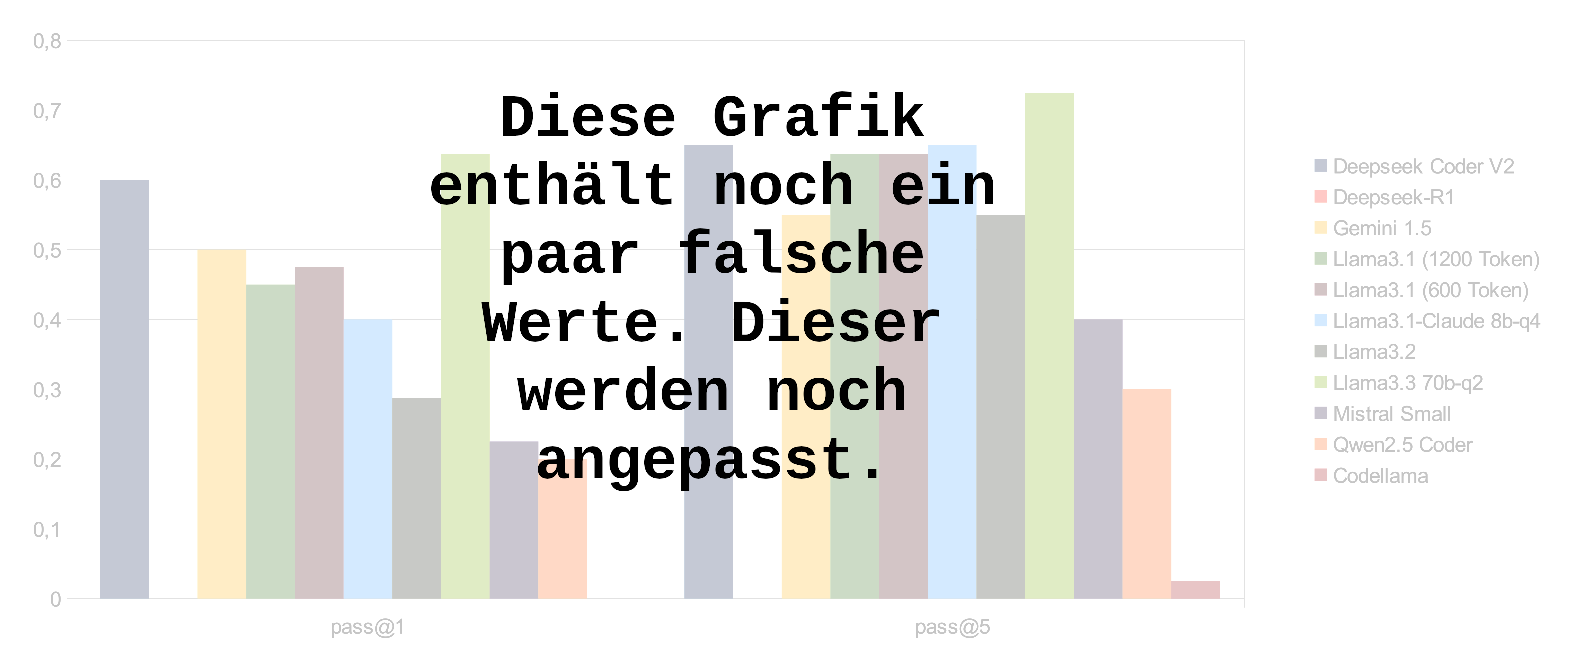
\includegraphics[width=\textwidth]{content/chapter_evaluation/images/llm_evaluation.eps}
	\centering
	\caption{Ergebnisse der pass@k-Methode für die Modelle}
	\label{img:pass_at_k_results_by_llm}
\end{figure}

Zwei weitere Modelle aus dem Open-Source-Bereich sind die Modelle \textit{Mistral-Small 22b} von der gleichnamigen Firma MistralAI und \textit{Qwen 2.5 Coder 32b}. Diese beiden Modelle schnitten im Vergleich nicht so gut ab. \vspace{0.2cm}

Das Modell \textit{Deepseek Coder V2 16b} welches an die Leistung von den Llama3.1 Modellen heranreicht.\vspace{0.2cm}
%Die Antworten von ChatGPT enthielten bei der ersten Abfrage Programmcode, alle weiteren Abfragen verwiesen auf den ersten Prompt. Eine Antwort ist in ?? dar gestellt, diese wurde in ähnlicher Weise immer wieder generiert.
%\hrulefill
%Der Code in deinem Kommentar ist identisch mit dem aktuellen Inhalt. Wenn du Än\-der\-ungen vornehmen möchtest, präzisiere bitte, was angepasst werden soll, und ich werde es umsetzen!
%\begin{flushright}
%	\textit{Generiert von ChatGPT 3.5}
%\end{flushright}
%\hrulefill

Ein weiteres Modell ist Gemini 15. von Google. Im Gegensatz zu den anderen Modellen, bringt Gemini nicht immer nur eine Lösung des Problems, sondern bietet weitere Ansätze, welche ebenfalls für das jeweilige Problem interessant sein könnten. Im folgenden Beispiel sind die verschiedenen Vorschläge des Modells in den Listings \ref{lst:gemini_result_php-3_1} bis \ref{lst:gemini_result_php-3_4} dargestellt, die beim PHP Problem 3 gefordert wurden. Die Aufgabenstellung in Kurzform war: \texttt{Gib den größten gemeinsamen Teiler von zwei ganzen Zahlen a und b zurück.}

\begin{lstlisting}[language=PHP,label=lst:gemini_result_php-3_1,caption={Gemini Ergebnis für das PHP-3 Problem Version 1}]
function greatestCommonDivisorRecursive($a, $b) {
  if ($b === 0) {
    return $a;
  } else {
    return greatestCommonDivisorRecursive($b, $a % $b);
  }
}
\end{lstlisting}

Neben den geforderten Lösung gab Gemini noch weitere Lösungsvorschläge aus. Das Listing \ref{lst:gemini_result_php-3_2} zeigt einen zweiten Lösungsansatz.\vspace{0.2cm}

\begin{lstlisting}[
	language=PHP,
	label=lst:gemini_result_php-3_2,
	caption={Gemini Ergebnisse für das PHP-3 Problem Version 2}
]
function greatestCommonDivisorBinary($a, b) {
  if ($a == 0) return $b;
  if ($b == 0) return $a;

  // Ensure a is odd
  if ($a % 2 == 0 && $b % 2 == 0)
    return 2 * greatestCommonDivisorBinary($a / 2, $b / 2);
  if ($a % 2 == 0) return greatestCommonDivisorBinary($a / 2, $b);
  if ($b % 2 == 0) return greatestCommonDivisorBinary($a, $b / 2);

  // a and b are odd
  if ($a > $b) return greatestCommonDivisorBinary($a - $b, b);
  return greatestCommonDivisorBinary($b - a, a);
}
\end{lstlisting}

Zu diesem Beispiel hat Gemini 1.5 noch weitere Lösungsansätze generiert. Diese sind in \ref{lst:gemini_result_php-3_3} und \ref{lst:gemini_result_php-3_4} zu sehen.

\begin{lstlisting}[
	language=PHP,
	label=lst:gemini_result_php-3_3,
	caption={Gemini Ergebnisse für das PHP-3 Problem Version 3}
]
function leastCommonMultiple(int $a, int $b): int {
  // kgV(a, b) = (a * b) / ggT(a, b)
  return abs($a * $b) / greatestCommonDivisor($a, $b);
}
\end{lstlisting}

\begin{lstlisting}[
	language=PHP,
	label=lst:gemini_result_php-3_4,
	caption={Gemini Ergebnisse für das PHP-3 Problem Version 4}
]
function greatestCommonDivisorMultiple(int ...$numbers): int {
  // ggT von mehreren Zahlen
  return array_reduce($numbers, 'greatestCommonDivisor');
}
\end{lstlisting}

Einige Aufgaben wurden von Gemini aber wie ein Chat behandelt. So hat das Modell Antworten generiert, die einer Konversation mit einem Chatbot ähneln, so wurde beispielsweise der folgende Text generiert, der einen Bezug zur zuvor gegebenen Antwort des Modells herstellt.

\hrulefill

\texttt{function greatestCommonDivisorRecursive(\$a, \$b) \{}

\texttt{\hspace{0.6cm} // ... (Rest der Funktion bleibt ähnlich)}

\texttt{\}}

\hrulefill

\begin{flushright}
	\textit{Generiert von Gemini 1.5}
\end{flushright}

Diese generierten Codeausschnitte haben die Tests nicht bestanden und wirken sich somit negativ auf die Auswertung aus.

\subsection{Nachteile der Evaluierung}
Es wird geprüft, ob der Code ohne Fehler ausführbar ist und die richtigen Ergebnisse liefert. Was dieser Test nicht evaluiert sind unter anderem vorhandene Codeerklärungen, Doc-Strings oder Code-Smells werden bei diesem Test nicht beachtet. Ebenso wird auch nicht der Codestandard geprüft.\vspace{0.2cm}

Benchmark prüfen, ob die Tests evtl. Fehler enthalten. Dies könnte sich beispielsweise in folgenden Probleme darstellen,

\begin{itemize}
	\item Tests sind falsch formuliert und die Abdeckung der geforderten Aufgabe wird nicht erfüllt, wodurch fehlerhafter generierter Code als korrekt bewertet wird.
	\item Fehler in den Musterlösungen können dazu führen, dass korrekte Lösungen als nicht bestanden gewertet werden.
	\item Mehrdeutige Aufgabenstellungen können ebenfalls das Ergebnis der Modelle negativ beeinflussen.
	\item Die Benchmark existieren bereit mehrere Jahre, sodass nicht ausgeschlossen werden kann, das Modelle explizit mit diesen Benchmarks trainiert wurden.
\end{itemize}

%--- Optimierung --------------------------------------------------------------------------------


\section{Optimierung der Ergebnisse}
Als Ziel der Optimierung gilt das die LLMs effizienten, präzisen und korrekten Code zu generieren. Ein Ansatz dies zu erreichen ist die Prompts zur Codegenerierung mithilfe einer LLMs zu erstellen oder zu verbessern.


% https://ki-techlab.de/ki-news/evaluierung-grosser-sprachmodelle-ein-technischer-leitfaden/

%\begin{tcolorbox}[
%	enhanced,
%	colback=BhtColorYellow!5!white,
%	colframe=BhtColorYellow!75!black,
%	title= HTML Startseite
%	]
%	Text in der Box
%\end{tcolorbox}

%\begin{tcolorbox}[
%	enhanced,
%	colback=BhtGrey!5!white,
%	colframe=BhtGrey!75!black!50,
%	title= ChatGPT 3.5
%	]
% Text in der Box
%\end{tcolorbox}
